%%%%%%%%%%%%%%%%%%%%%%%%%%%%%%%%%%%%%%%%%%%%
\section{Conclusions}


%%%%%%%%%%%%%%%%%%%%%%%%%%%%%%%%%%%%%%%%%%%%%%%%%%%%%%%%
{
%\paper{Xochicale 2019 in {\bf PhD thesis}}

\begin{frame}{Conclusions and future work}

\textbf{Take away messages}
\begin{itemize}
\item Nonlinear analysis tools can quantify different
data time-series. 
\item Shannon entropy with 3D plot surfaces of RQA appear to be robust for real-word data (i.e. different time series
structures, window length size and levels of smoothness).
\item Therefore, Shannon entropy would be a potential good tool to quantify complexity of movement.
%\item Smoothing raw time series can create well defined trajectories
%or patterns in RSS or RP, however such increase of smoothness 
%can also create more complex (i.e. not well defined) trajectories
%or patterns in nonlinear analysis. 

\end{itemize}

\textbf{Investigate}
\begin{itemize}
	\item other methodologies for state space reconstruction,
	\item the robustness of Entropy measurements with RQA, and 
	\item variability in perception of velocity.
\end{itemize}




\end{frame}
}





{
{
\paper{Zia et al., 2017 in {\bf Computer Assisted Radiology and Surgery};
Mori 2012 in {\bf Development and Learning and Epigenetic Robotics};
Mitsukura et al., 2017 in {\bf Electroencephalography}; 
Marwan et al. 2019 in {\bf http://recurrence-plot.tk/}
}
\begin{frame}{Applications of Nonlinear Dynamics}
    \vspace{-02mm}
    \begin{figure}
        \centering
        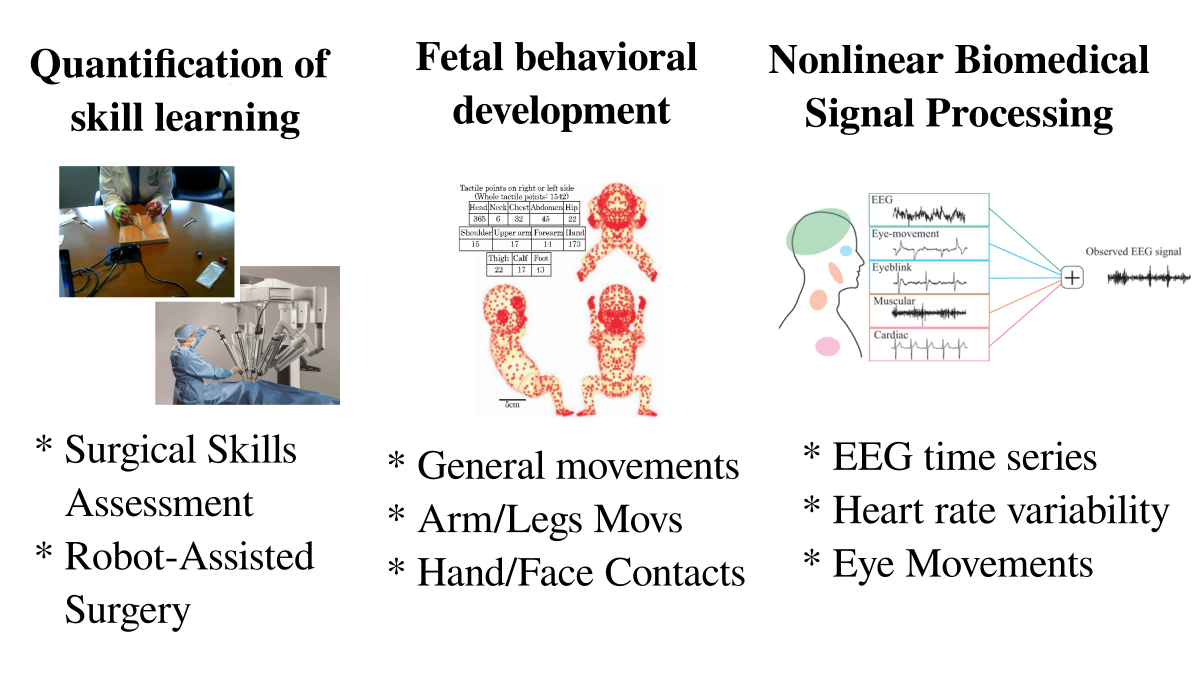
\includegraphics[width=0.9\linewidth]{./figs/applications/versions/drawing-v00.png}
	%\caption{} 
   \end{figure}
	
\end{frame}
}

